\chapter{Experimentação e Avaliação} 
\label{chap:Chapter04}

A avaliação da aplicação é essencial para garantir sua eficácia, acessibilidade e usabilidade. Este capítulo descreve o plano de experimentação e avaliação adotado para testar e validar a aplicação. Para isso, será utilizado o método GQM (Goals, Questions, Metrics), além de outros testes de acessibilidade.

\section{Metodologia de Avaliação}

\subsection{Hipótese de Investigação}

A avaliação do projeto terá como base a seguinte hipótese: O uso da do simulador da Máquina Braille melhora a aprendizagem do Braille e do uso da Máquina Braille.

\subsection{Goals, Questions, Metrics}

O método \textit{"Goal Question Metric"} (GQM) é uma abordagem que ajuda organizações a medir seus processos de forma eficaz \parencite{ARTICLE13}. Ele começa com a definição clara dos objetivos da organização e de seus projetos. Em seguida, esses objetivos são relacionados a perguntas específicas que orientam a coleta de dados relevantes. Finalmente, os dados coletados são analisados para interpretar se os objetivos foram alcançados.

\begin{figure}[h]
    \centering
    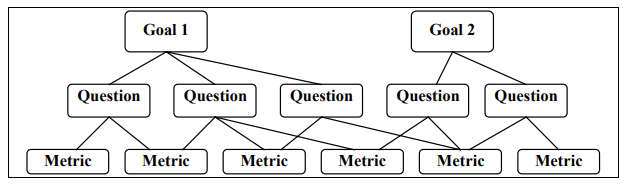
\includegraphics[scale=0.5]{ch04/assets/gqm.png}
    \decoRule
    \caption[Goal, Question, Metric]{Goal, Question, Metric \parencite{ARTICLE13}}
    \label{fig:ch02-gqm}
\end{figure}

A metodologia GQM será utilizada para definir objetivos claros, formular questões relevantes e identificar métricas adequadas para medir o desempenho da aplicação. Na tabela \ref{tab:GQM}, são apresentados os objetivos, as perguntas e as métricas que serão utilizadas na avaliação.

\begin{table}[h]
    \caption{Goals, Questions and Metrics}
    \label{tab:GQM}
    \centering
    \begin{tabular}{|p{0.2\linewidth}|p{0.35\linewidth}|p{0.35\linewidth}|} \hline 
         \textbf{Goal} & \textbf{Questions} & \textbf{Metrics} \\ \hline
        \textbf{(G1) Avaliar a Usabilidade da Aplicação} & 
        \begin{itemize}
            \item (Q1) Os usuários conseguem utilizar a aplicação de forma intuitiva?
            \item (Q2) A interface da aplicação é amigável e fácil de usar?
        \end{itemize} & 
        \begin{itemize}
            \item (M1) Número de erros cometidos pelos usuários ao tentar usar as funcionalidades básicas.
            \item (M2) Tempo médio para completar uma lição ou tarefa específica.
            \item (M3) Pontuação média em questionários de satisfação dos usuários.
            \item (M4) Comentários qualitativos sobre a experiência de uso.
        \end{itemize} \\ \hline
        
        \textbf{(G2) Avaliar a Eficácia no Aprendizado do Braille} & 
        \begin{itemize}
            \item (Q3) A aplicação ajuda os usuários a aprender e praticar Braille de maneira eficaz?
            \item (Q4) Os usuários conseguem transitar do uso da aplicação para o uso de uma máquina Braille real de forma eficiente?
        \end{itemize} & 
        \begin{itemize}
            \item (M5) Percentual de acertos em testes de conhecimento de Braille antes e depois do uso da aplicação.
            \item (M6) Tempo médio para os usuários completarem lições com sucesso ao longo do tempo.
            \item (M7) Feedback dos usuários sobre a transição para a máquina Braille real.
            \item (M8) Número de tentativas necessárias para os usuários realizarem corretamente tarefas em uma máquina Braille real após praticarem com a aplicação.
        \end{itemize} \\ \hline
        
        \textbf{(G3) Avaliar a Acessibilidade da Aplicação} & 
        \begin{itemize}
            \item (Q5) A aplicação é acessível para pessoas com deficiência visual?
            \item (Q6) Os recursos de acessibilidade, como feedback sonoro, são eficazes?
        \end{itemize} & 
        \begin{itemize}
            \item (M9) Conformidade com as Diretrizes de Acessibilidade para Conteúdo Web (WCAG) 2.1.
            \item (M10) Resultados de testes de acessibilidade automatizados e manuais.
            \item (M11) Feedback qualitativo dos usuários sobre os recursos de acessibilidade.
        \end{itemize} \\ \hline
    \end{tabular}
\end{table}

A figura \ref{fig:ch04-map-gqm} mostra a relação dos objetivos, questionamentos e métricas.

\begin{figure}[h]
    \centering
    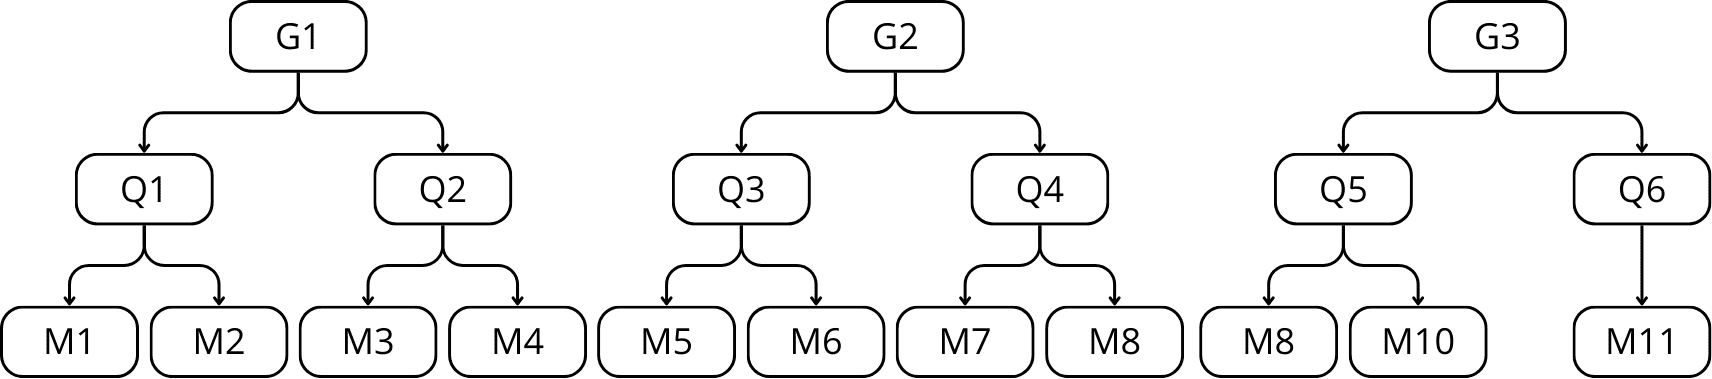
\includegraphics[scale=0.3]{ch04/assets/map-gqm.png}
    \decoRule
    \caption[Mapa do GQM]{Mapa do GQM}
    \label{fig:ch04-map-gqm}
\end{figure}

\section{Procedimentos de avaliação}

\subsection{Seleção de Participantes}

Os participantes dos testes serão selecionados visando obter uma amostra diversificada que represente diferentes perfis de usuários e ofereça insights abrangentes sobre a usabilidade, eficácia no aprendizado e acessibilidade da aplicação. Serão consideradas três categorias principais de participantes:

\begin{enumerate}
    \item \textbf{Usuários com Deficiência Visual:} Esta categoria abrangerá indivíduos que são cegos ou possuem baixa visão, tanto aqueles que adquiriram a deficiência recentemente quanto os que já possuem familiaridade com o Braille. A inclusão destes participantes permitirá avaliar como a aplicação atende às necessidades específicas de pessoas com deficiência visual, além de sua eficácia em promover o aprendizado e a prática do Braille de forma inclusiva.

    \item \textbf{Usuários sem Deficiência Visual:} Esta categoria englobará pessoas sem deficiência visual que desejam aprender Braille por motivos educacionais, profissionais ou de interesse pessoal. A participação destes usuários fornecerá insights sobre a experiência daqueles que estão sendo introduzidos ao Braille pela primeira vez, bem como sua percepção sobre a usabilidade e eficácia da aplicação.

    \item \textbf{Instrutores e Educadores:} Professores e instrutores especializados no ensino de Braille serão convidados a participar dos testes para oferecer uma perspectiva educacional sobre a aplicação. Esses profissionais possuem conhecimento especializado sobre as melhores práticas de ensino do Braille e podem oferecer insights sobre a eficácia pedagógica da aplicação, sua adequação para uso em ambientes educacionais e possíveis melhorias para otimizar a experiência de aprendizado dos alunos.
\end{enumerate}

Será assegurado que todos os participantes estejam confortáveis e seguros ao participarem dos testes, e qualquer preocupação com acessibilidade será atendida para garantir uma participação equitativa e significativa.

\subsection{Ambiente de Teste}

Os testes serão realizados em um ambiente que forneça condições ideais para a avaliação da aplicação. O ambiente de teste para cada usuário será em uma sala equipada com um computador de mesa com a aplicação, que conterá um teclado, um mouse, fones de ouvido ou caixas de som (dependendo da preferência do usuário).

O ambiente de teste será projetado para garantir a privacidade e o conforto dos participantes. Será reservado um tempo adequado para que os participantes possam familiarizar-se com a aplicação antes de iniciar os testes.

\subsection{Procedimentos de testes}

\subsubsection{Testes de Usabilidade}

Os testes de usabilidade serão conduzidos com o objetivo de avaliar a facilidade de uso e a intuitividade da aplicação. Os participantes serão solicitados a realizar uma série de tarefas específicas, como escrever palavras simples em Braille, utilizar a funcionalidade de quebra de linha e navegar pelo texto. 

Durante a realização dessas tarefas, serão registrados o número de erros cometidos pelos usuários e o tempo necessário para completar cada tarefa. Além disso, ao final dos testes, os participantes preencherão um questionário de satisfação, avaliando de 1 a 5 os seguintes aspectos da interface e usabilidade da aplicação: 

\begin{itemize}
    \item Clareza das instruções;
    \item Organização das funcionalidades
    \item Facilidade de aprendizado
\end{itemize}

\subsubsection{Testes de Eficácia no Aprendizado}

Os testes de eficácia no aprendizado têm como objetivo avaliar a capacidade da aplicação de facilitar o aprendizado do Braille e melhorar as habilidades dos usuários na escrita em Braille. Para isso, os participantes realizarão um teste de conhecimento antes e após o uso da aplicação, nos quais serão apresentadas questões relacionadas ao contexto do Braille e da Máquina Braille:

\begin{enumerate}
    \item Qual é a principal função do Sistema Braille?
    \item Quantos pontos compõem uma célula Braille?
    \item A Máquina Braille é formada por quais teclas?
    \item Quais pontos formam cada letra do seu nome no Sistema Braille?
    \item Qual sinal é utilizado para representar os números no sistema Braille?
    \item Quais são os sinais de pontuação mais comuns no Braille e como são representados?
    \item Como a máquina de escrever em Braille facilita a produção de textos em Braille?
\end{enumerate}

A diferença entre as pontuações obtidas nos dois testes indicará o progresso no aprendizado após a utilização da aplicação. Além disso, os participantes completarão uma série de lições e exercícios dentro da aplicação, com o progresso sendo monitorado ao longo do tempo para avaliar a eficácia do aprendizado.

\subsubsection{Testes de Acessibilidade}

Os testes de acessibilidade visam garantir que a aplicação seja acessível para pessoas com deficiência visual, permitindo que elas a utilizem de forma eficiente e autônoma. A acessibilidade será avaliada em conformidade com as Diretrizes de Acessibilidade para Conteúdo Web (WCAG) 2.1, utilizando tanto ferramentas automatizadas quanto inspeção manual. Serão verificados aspectos como o contraste de cores, a legibilidade do texto, a navegabilidade por meio de teclado e a compatibilidade com leitores de tela. 

Além disso, serão coletados feedbacks qualitativos dos usuários sobre a acessibilidade da aplicação, focalizando na eficácia dos recursos de feedback sonoro e na facilidade de navegação.
